\section{修订后的点预测结果与消融比较}
本章采用修订求解器产生的CSI300测试结果，共1919个预测原点，2018年5月3日至2026年3月30日。XGBoost沿用已逐点匹配历史预测的配置及列抽样；HAR、GARCH重新估计。DEC使用解析梯度和确定性多起点估计，新增XGB-AR作为不含EPU的残差修正对照。历史结果保留在项目原结果目录；本章数值来自\path{results/revised/}，不与旧版混用。

\subsection{点预测损失}
\begin{table}[htbp]\centering\caption{CSI300修订点预测结果，N=1919}\label{tab:forecast_metrics}
\begin{tabular}{lrrr}\toprule
模型 & MSE & MAE & QLIKE \\
\midrule
HAR & 4.905206 & 1.724860 & 3.905553 \\
GARCH(1,1) & 7.375868 & 1.983865 & 1.564183 \\
XGB-Market & 5.099716 & 1.763086 & 4.951636 \\
XGB-AR & 5.094169 & 1.758021 & 4.705936 \\
DEC & 5.112644 & 1.725558 & 3.536964 \\
\bottomrule\end{tabular}\end{table}

MSE、MAE和QLIKE均越低越好。HAR的对数MSE和MAE最低，GARCH的QLIKE最低。DEC相对XGB-Market的QLIKE下降约28.57\%，MAE下降约2.13\%，但MSE上升约0.25\%。因此不能声称复杂修正全面改进基准。对数目标反变换与直接方差预测的差异也影响排序，不能全部解释为模型结构的优劣。

相对XGB-AR，DEC的QLIKE从4.705936降至3.536964，MAE从1.758021降至1.725558，MSE从5.094169升至5.112644。这提供加入EPU后损失依赖的增量预测比较；它不证明政策不确定性的外生因果作用，也不证明月度数据在当时实时可得。
\begin{figure}[htbp]\centering
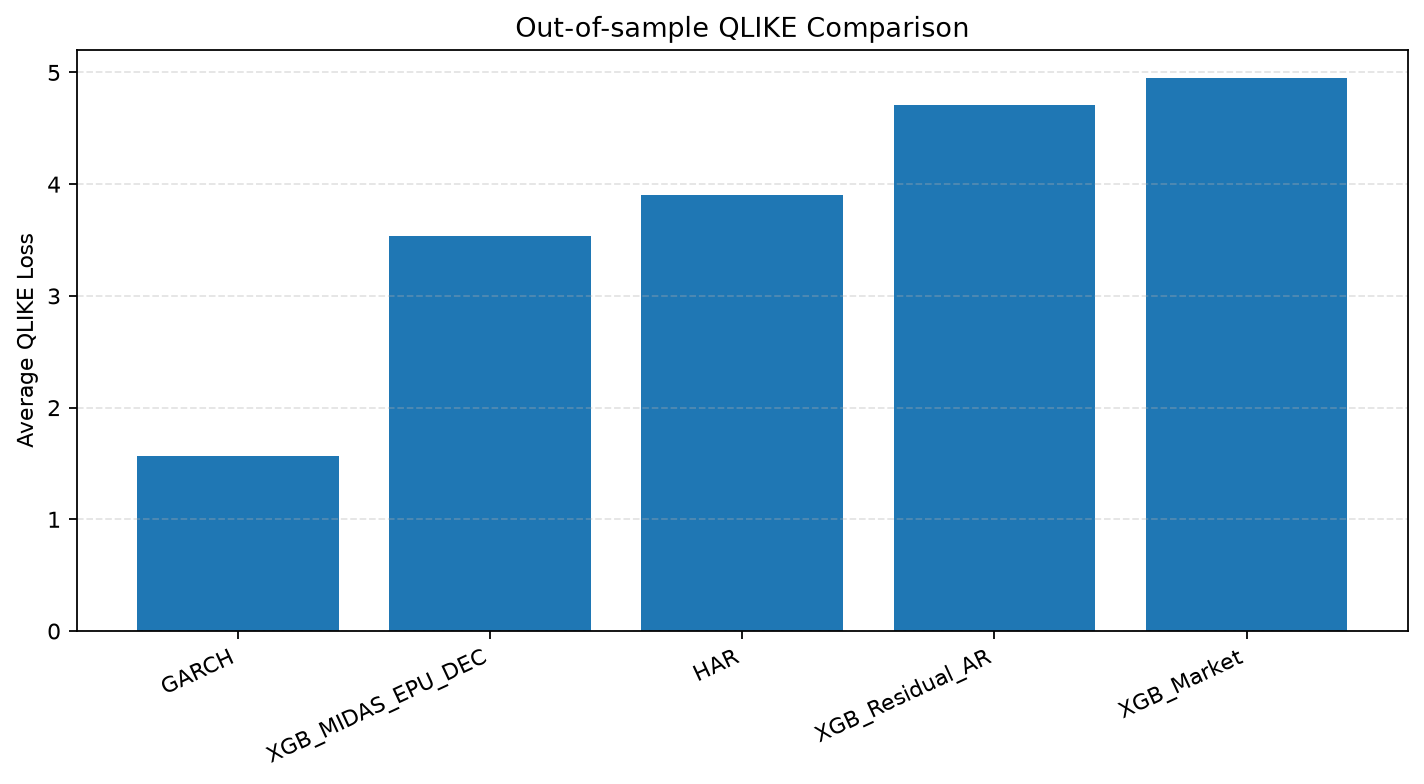
\includegraphics[width=.88\textwidth]{../../results/revised/csi300/fig_metrics_bar.png}
\caption{CSI300修订结果：五模型的QLIKE}\label{fig:metrics_bar}\end{figure}

\subsection{预测路径与累计损失}
近期路径及累计QLIKE差见图\ref{fig:prediction_series}和图\ref{fig:cumulative_qlike}。累计差定义为基准损失减DEC损失，曲线上升表示累计差向DEC有利方向变化；累计曲线不证明每一天均改善，也不能排除极端日期的影响。路径较平滑不能单独证明模型有效。
\begin{figure}[htbp]\centering
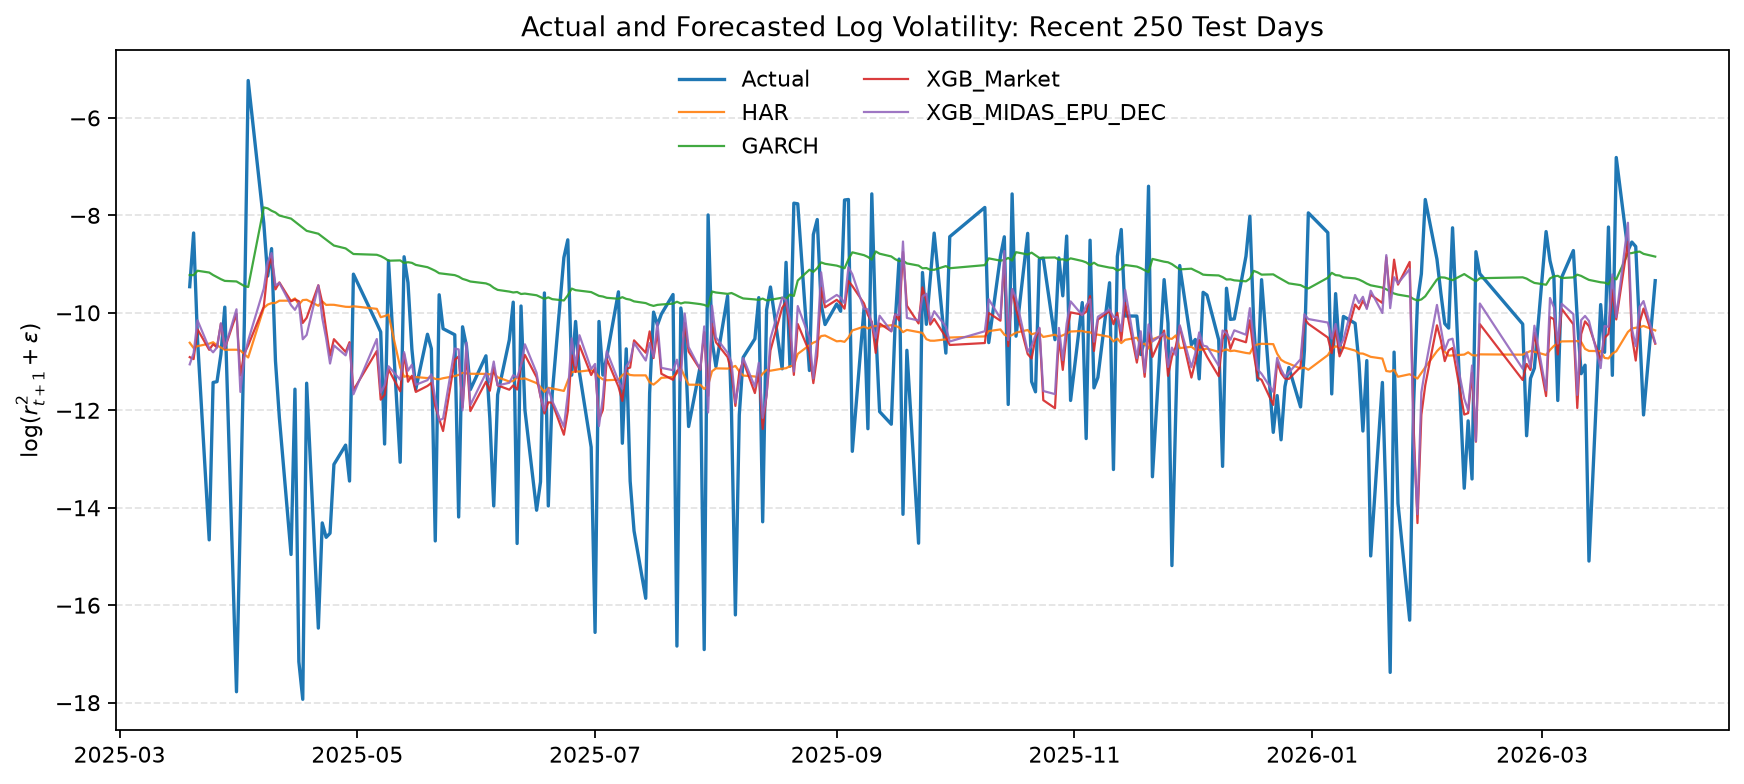
\includegraphics[width=.88\textwidth]{../../results/revised/csi300/fig_prediction_series_recent.png}
\caption{修订DEC与三个基准的近期预测路径}\label{fig:prediction_series}\end{figure}
\begin{figure}[htbp]\centering
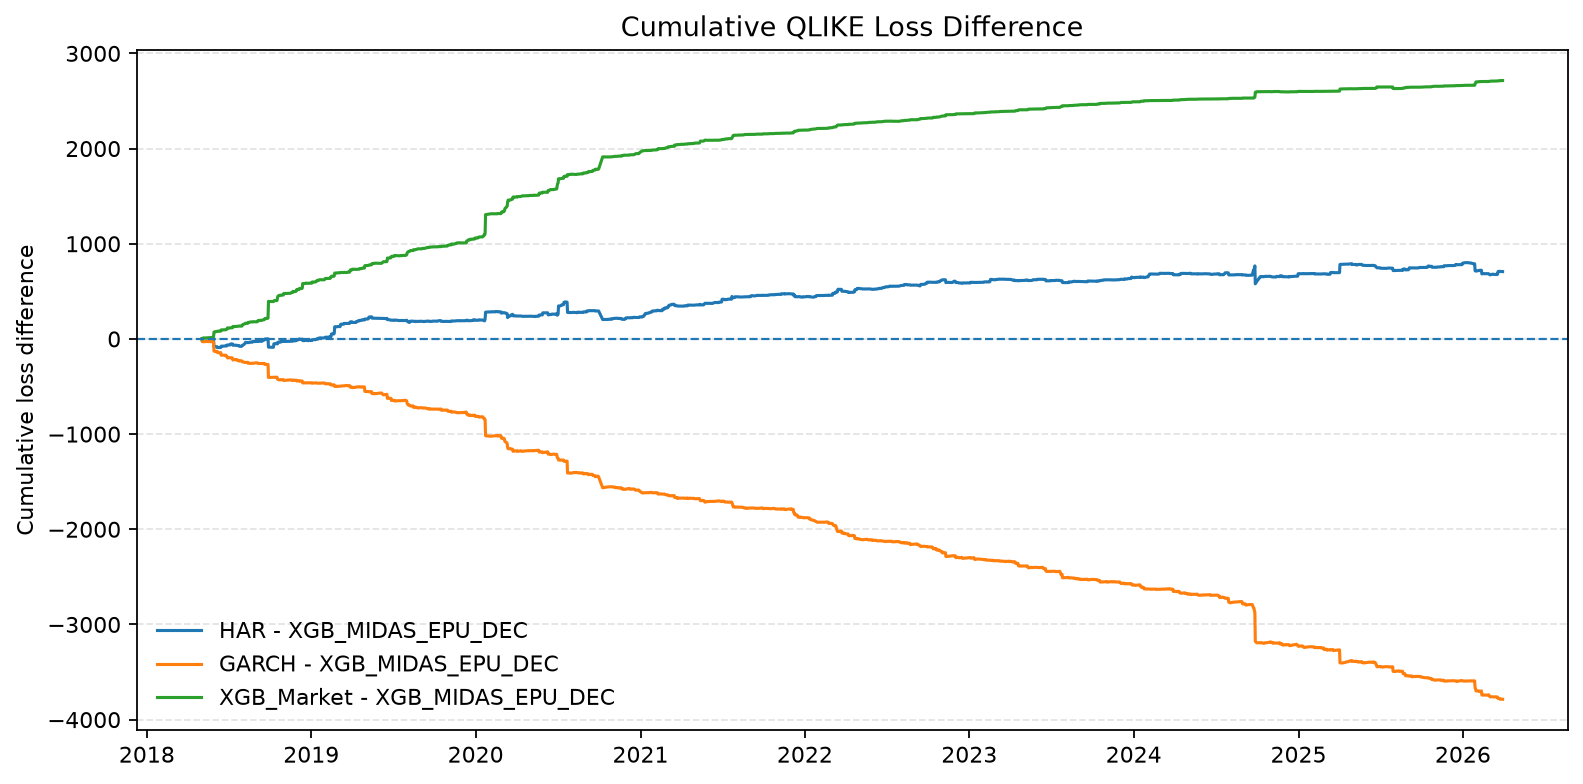
\includegraphics[width=.88\textwidth]{../../results/revised/csi300/fig_cumulative_qlike_diff.png}
\caption{修订DEC相对三基准的累计QLIKE差}\label{fig:cumulative_qlike}\end{figure}

\subsection{损失差诊断与统计解释}
表\ref{tab:hypothesis_tests}给出CSI300六项比较。正的平均损失差表示DEC更低；Holm调整覆盖三个市场的全部18项。MAE和QLIKE的差异在这些探索性参考值下较明确，MSE差异没有相应证据。模型选择及近似嵌套限制仍然存在，不能把调整后的$p$值当作完全有效的确认性检验。
\begin{table}[htbp]\centering\caption{CSI300损失差的探索性HAC诊断}\label{tab:hypothesis_tests}
\begin{tabular}{llrrr}\toprule 比较对象 & 损失 & 均值差 & HAC标准误 & Holm $p$\\\midrule
XGB-Market & MSE & -0.012928 & 0.041430 & 1\\
XGB-Market & MAE & 0.037528 & 0.008207 & 6.73e-05\\
XGB-Market & QLIKE & 1.414672 & 0.197725 & 1.43e-11\\
XGB-AR & MSE & -0.018475 & 0.035984 & 1\\
XGB-AR & MAE & 0.032464 & 0.007137 & 7.01e-05\\
XGB-AR & QLIKE & 1.168972 & 0.160859 & 6.61e-12\\
\bottomrule\end{tabular}\end{table}

\subsection{规格选择、权重及数值敏感性}
CSI300仍选24个月指数Almon。规格选择段的参数见表\ref{tab:midas_spec}，实际测试期每60条重新估计，因此图\ref{fig:midas_weights}不是固定全样本经济效应。参数触及边界也提示权重形状依赖约束，不能据其解释政策传导期限。
\begin{table}[htbp]\centering\caption{CSI300修订验证集所选规格}\label{tab:midas_spec}
\begin{tabular}{lrrrr}\toprule 权重族 & K & $\theta_1$ & $\theta_2$ & 验证MSE\\\midrule
指数Almon & 24 & 5.000000 & -4.488853 & 5.722685\\\bottomrule\end{tabular}\end{table}
\begin{figure}[htbp]\centering
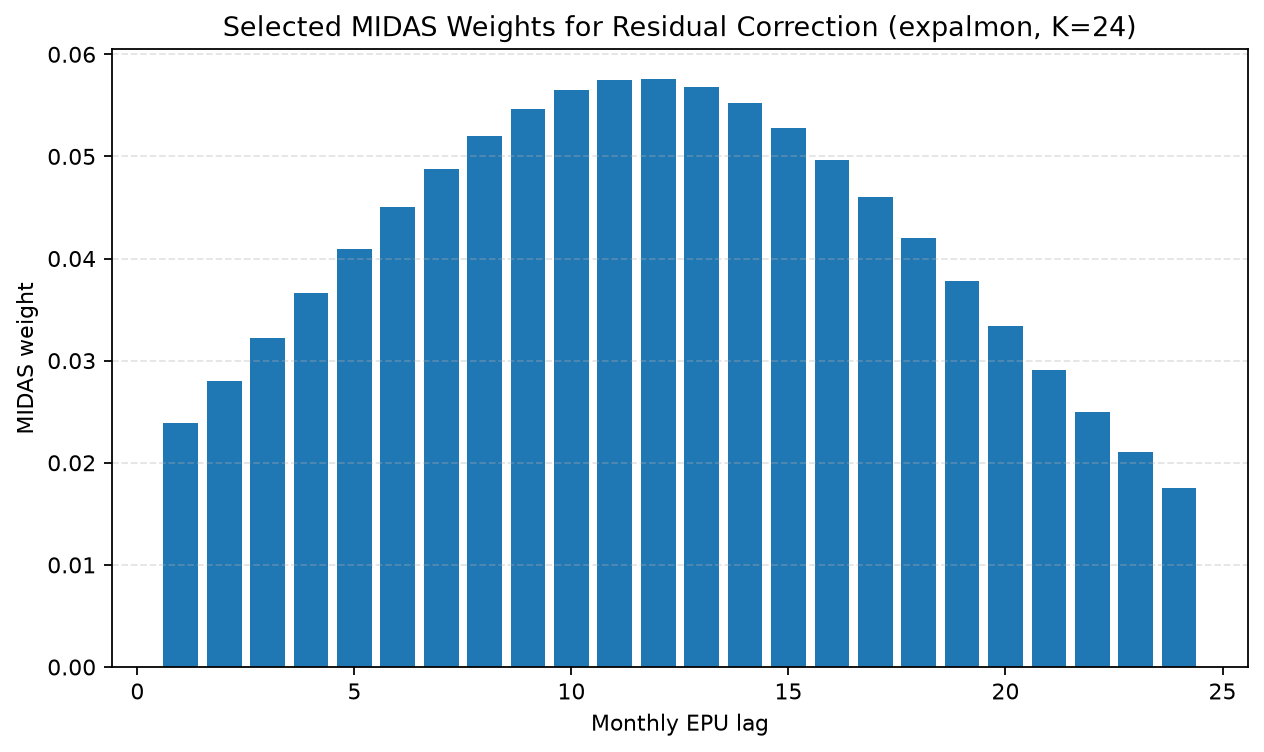
\includegraphics[width=.88\textwidth]{../../results/revised/csi300/fig_midas_weights.png}
\caption{修订后的CSI300验证选择权重}\label{fig:midas_weights}\end{figure}

旧存档DEC的MSE为5.112383、QLIKE为3.538317；修订后分别为5.112644和3.536964。MSE略差、QLIKE略好，不构成全面提升。修订理由是明确的数值估计缺陷和可复核的优化诊断，而不是追求较好看的测试成绩。附录和项目记录分别列出旧环境复现差异、固定规格控制以及新方法的跨依赖检查。

\subsection{本章小结}
CSI300支持保留传统基准，同时表明DEC的样本优势依赖评价损失。新增消融使“含EPU的组合与仅含残差的组合有何不同”可以直接比较；结论仍限定于当前数据、回顾性设计和预先固定的本轮求解规则。对区间质量是否有改善，需要单独检验。
